\section{Erzeugung der Eingangsbilder}

Die Erzeugung von Eingangsbildern für unser neuronales Netz, war eines der ersten Probleme, welches wir gelöst haben. Testbilder zu suchen oder selbst zu erstellen kann sehr Zeitaufwendig sein. Aus diesem Grund haben wir zwei Matlab-Skripte geschrieben, die uns dieses Problem zukünftig abnehmen. Die beiden Dateien heißen 'GetPixelFeatureMatrix.m' und 'TestGetPixelFeatureMatrix.m'. Das 'PixelFeatureMatrix.m' erwartet als Eingang eine Merkmale-Matrix, die dann auf eine Pixel-Matrix skaliert wird. Darüber hinaus kann auch ein Rauschwert angegeben werden, um das neuronale Netz auf Rauschempfindlichkeit zu testen. Im Anschluss sind ein paar Bilder erzeugt worden mit unterschiedlichen Pixel- und Merkmalanzahlen. Bei den Kreuzdarstellungen wurde darüber hinaus die Rauscheinstellungen geändert.

\begin{figure}[hbt]
	\begin{minipage}{0.5 \textwidth}
		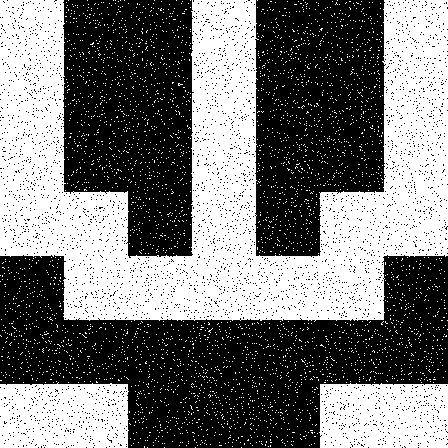
\includegraphics[width=\textwidth]{./Bilder/Auswertung/BeispielBilder/Picture_Example4_noise_10_pixelCnt_64_featureCnt_7}
		\caption{448x448, Rauschen 10}
		% \label{eindeutigerBezeichner}
	\end{minipage}
	\hfill
	\begin{minipage}{0.5 \textwidth}
		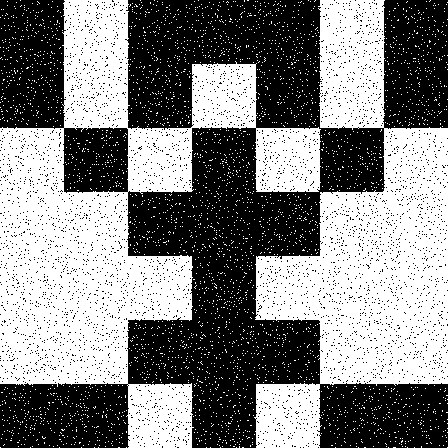
\includegraphics[width=\textwidth]{./Bilder/Auswertung/BeispielBilder/Picture_Example2_noise_10_pixelCnt_64_featureCnt_7}
		\caption{640x640, Rauschen 10}
		% \label{eindeutigerBezeichner}
	\end{minipage}
\end{figure}

\begin{figure}[hbt]
	\begin{minipage}{0.5 \textwidth}
		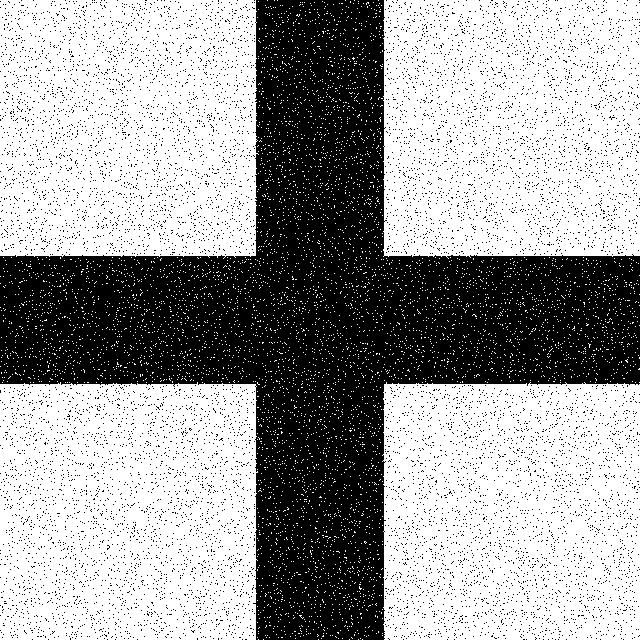
\includegraphics[width=\textwidth]{./Bilder/Auswertung/BeispielBilder/Picture_Crossing_noise_10_pixelCnt_128_featureCnt_5}
		\caption{640x640, Rauschen 10}
		% \label{eindeutigerBezeichner}
	\end{minipage}
	\hfill
	\begin{minipage}{0.5 \textwidth}
		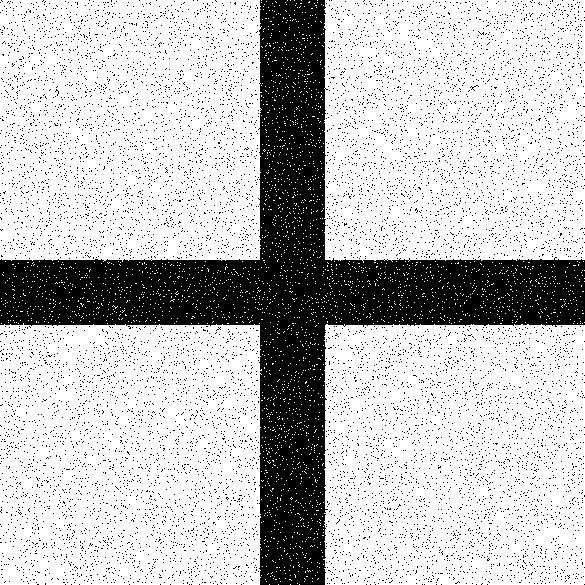
\includegraphics[width=\textwidth]{./Bilder/Auswertung/BeispielBilder/Picture_Crossing_noise_10_pixelCnt_65_featureCnt_9}
		\caption{585x585, Rauschen 10}
		% \label{eindeutigerBezeichner}
	\end{minipage}
\end{figure}

\begin{figure}[hbt]
	\begin{minipage}{0.5 \textwidth}
		
\includegraphics[width=\textwidth]{./Bilder/Auswertung/BeispielBilder/Picture_Line1_noise_10_pixelCnt_128_featureCnt_5}
		\caption{640x640, Rauschen 10}
		% \label{eindeutigerBezeichner}
	\end{minipage}
	\hfill
	\begin{minipage}{0.5 \textwidth}
		
\includegraphics[width=\textwidth]{./Bilder/Auswertung/BeispielBilder/Picture_Line2_noise_10_pixelCnt_128_featureCnt_5}
		\caption{640x640, Rauschen 10}
		% \label{eindeutigerBezeichner}
	\end{minipage}
\end{figure}

\begin{figure}[hbt]
	\begin{minipage}{0.5 \textwidth}
		
\includegraphics[width=\textwidth]{./Bilder/Auswertung/BeispielBilder/Picture_Crossing_noise_0_pixelCnt_128_featureCnt_5}
		\caption{640x640, Rauschen 0}
		% \label{eindeutigerBezeichner}
	\end{minipage}
	\hfill
	\begin{minipage}{0.5 \textwidth}
		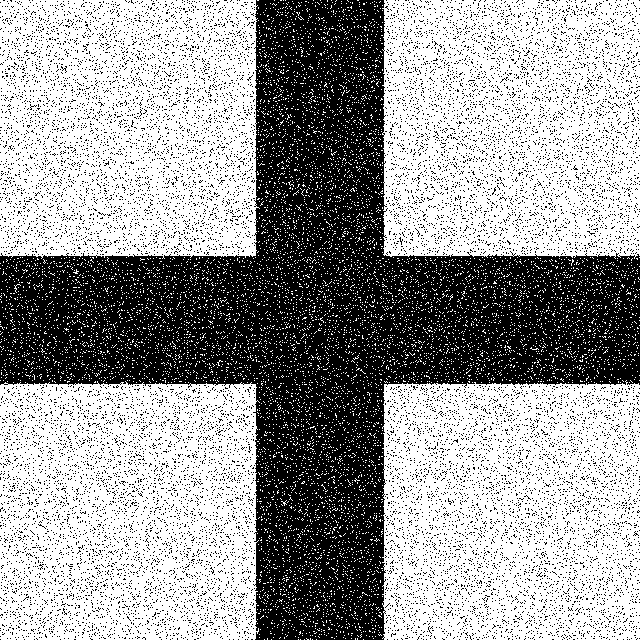
\includegraphics[width=\textwidth]{./Bilder/Auswertung/BeispielBilder/Picture_Crossing_noise_20_pixelCnt_128_featureCnt_5}
		\caption{640x640, Rauschen 20}
		% \label{eindeutigerBezeichner}
	\end{minipage}
\end{figure}

\begin{figure}[hbt]
	\begin{minipage}{0.5 \textwidth}
		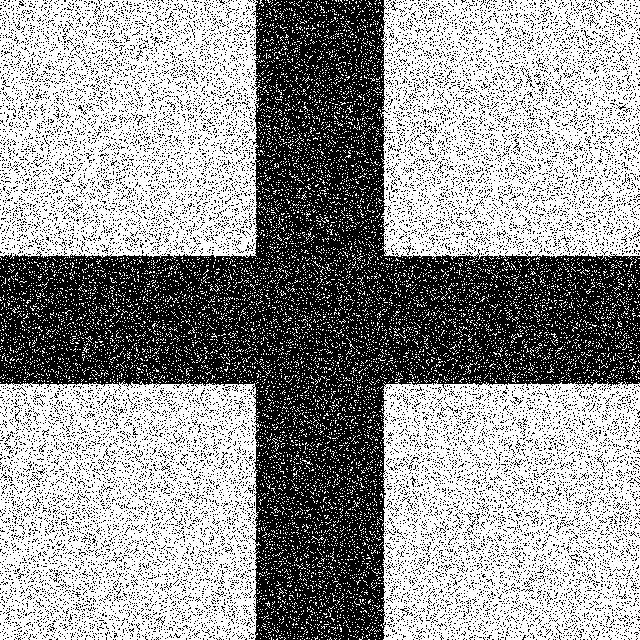
\includegraphics[width=\textwidth]{./Bilder/Auswertung/BeispielBilder/Picture_Crossing_noise_30_pixelCnt_128_featureCnt_5}
		\caption{640x640, Rauschen 30}
		% \label{eindeutigerBezeichner}
	\end{minipage}
	\hfill
	\begin{minipage}{0.5 \textwidth}
		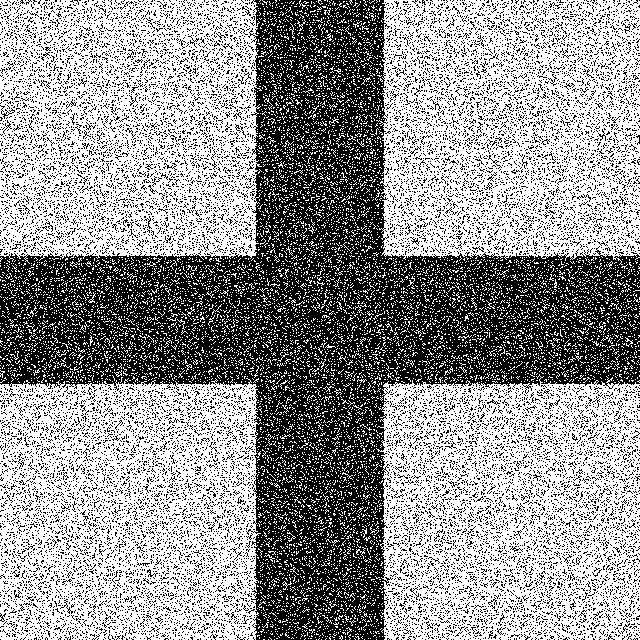
\includegraphics[width=\textwidth]{./Bilder/Auswertung/BeispielBilder/Picture_Crossing_noise_40_pixelCnt_128_featureCnt_5}
		\caption{640x640, Rauschen 40}
		% \label{eindeutigerBezeichner}
	\end{minipage}
\end{figure}

\begin{figure}[hbt]
	\begin{minipage}{0.5 \textwidth}
		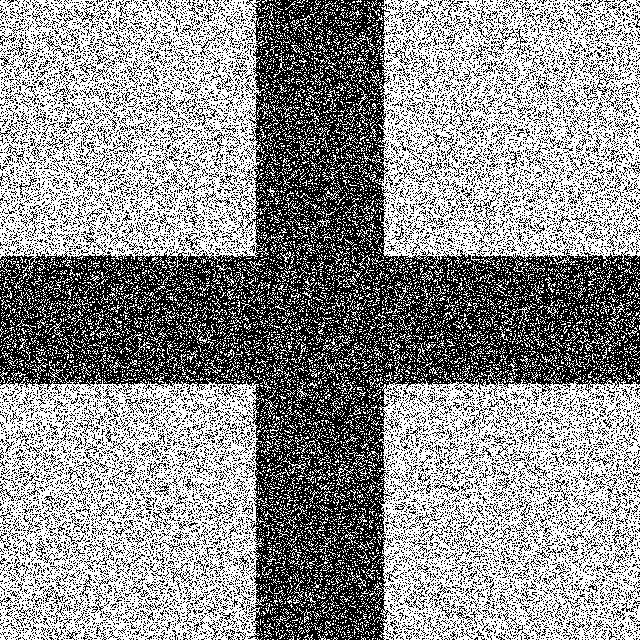
\includegraphics[width=\textwidth]{./Bilder/Auswertung/BeispielBilder/Picture_Crossing_noise_50_pixelCnt_128_featureCnt_5}
		\caption{640x640, Rauschen 50}
		% \label{eindeutigerBezeichner}
	\end{minipage}
	\hfill
	\begin{minipage}{0.5 \textwidth}
		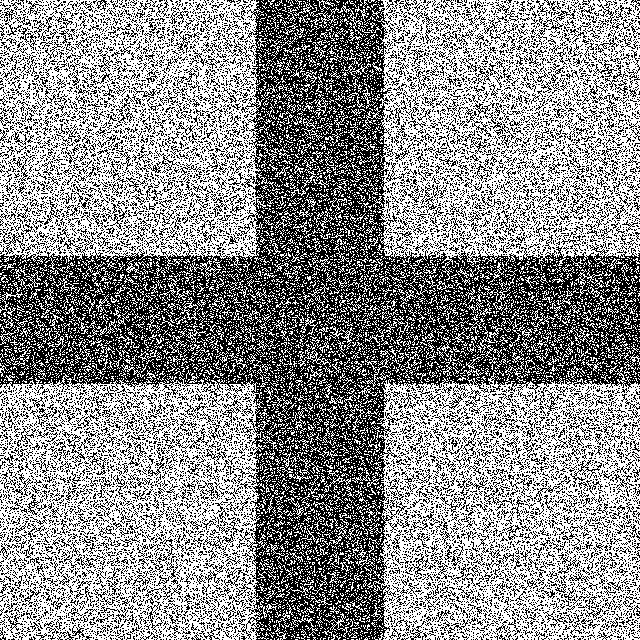
\includegraphics[width=\textwidth]{./Bilder/Auswertung/BeispielBilder/Picture_Crossing_noise_60_pixelCnt_128_featureCnt_5}
		\caption{640x640, Rauschen 60}
		% \label{eindeutigerBezeichner}
	\end{minipage}
\end{figure}

\begin{figure}[hbt]
	\begin{minipage}{0.5 \textwidth}
		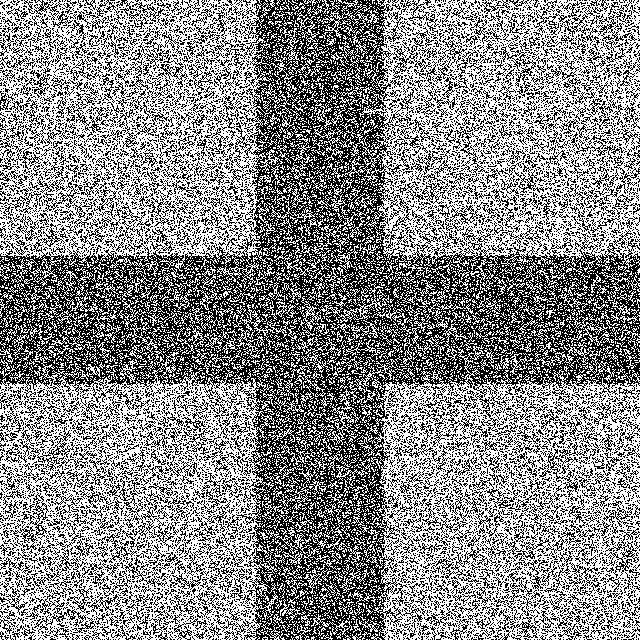
\includegraphics[width=\textwidth]{./Bilder/Auswertung/BeispielBilder/Picture_Crossing_noise_70_pixelCnt_128_featureCnt_5}
		\caption{640x640, Rauschen 70}
		% \label{eindeutigerBezeichner}
	\end{minipage}
	\hfill
	\begin{minipage}{0.5 \textwidth}
		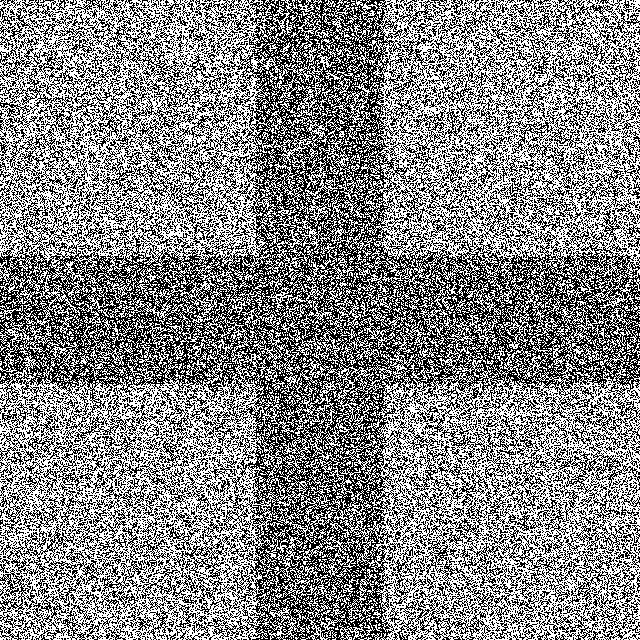
\includegraphics[width=\textwidth]{./Bilder/Auswertung/BeispielBilder/Picture_Crossing_noise_80_pixelCnt_128_featureCnt_5}
		\caption{640x640, Rauschen 80}
		% \label{eindeutigerBezeichner}
	\end{minipage}
\end{figure}

\begin{figure}[hbt]
	\begin{minipage}{0.5 \textwidth}
		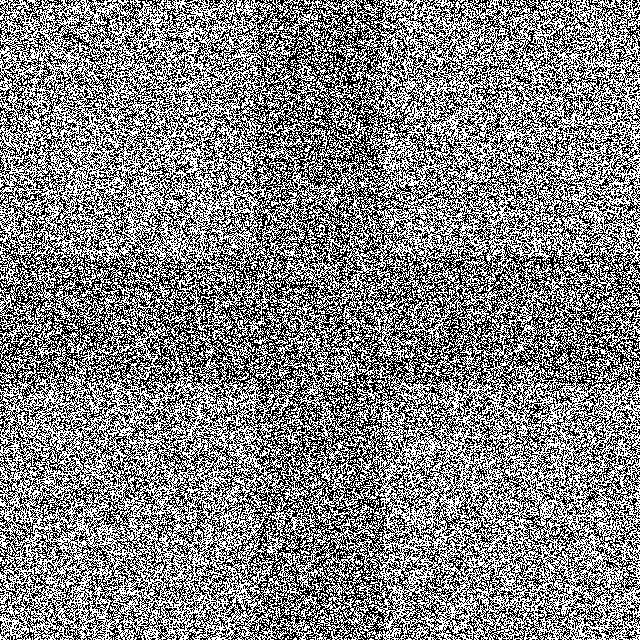
\includegraphics[width=\textwidth]{./Bilder/Auswertung/BeispielBilder/Picture_Crossing_noise_90_pixelCnt_128_featureCnt_5}
		\caption{640x640, Rauschen 90}
		% \label{eindeutigerBezeichner}
	\end{minipage}
	\hfill
	\begin{minipage}{0.5 \textwidth}
		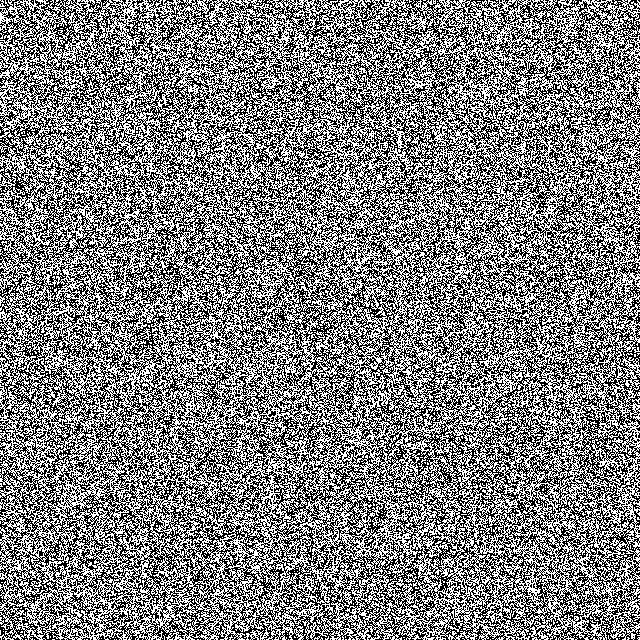
\includegraphics[width=\textwidth]{./Bilder/Auswertung/BeispielBilder/Picture_Crossing_noise_100_pixelCnt_128_featureCnt_5}
		\caption{640x640, Rauschen 100}
		% \label{eindeutigerBezeichner}
	\end{minipage}
\end{figure}

\begin{figure}[hbt]
	\centering
	
\includegraphics[width=0.7\linewidth]{./Bilder/Auswertung/BeispielBilder/Picture_Example1_noise_10_pixelCnt_128_featureCnt_5}
	\caption{640x640, Rauschen 10}
	% \label{eindeutigerBezeichner}
\end{figure}